\documentclass[
  10pt,
  aspectratio=169,
  utf8,
  xcolor={dvipsnames}
]{beamer}

\usetheme[
  progressbar=foot,
  sectionpage=progressbar,
  subsectionpage=progressbar,
  numbering=fraction
]{metropolis}
\usefonttheme{metropolis}
\usecolortheme{spruce}
\setbeamercolor{progress bar}{fg=MidnightBlue, bg=LightSteelBlue}
\setbeamercolor{title}{fg=MidnightBlue}
\setbeamercolor{frame title}{fg=MidnightBlue}
\setbeamercolor{structure}{fg=MidnightBlue}

\usepackage{booktabs}
\usepackage{graphicx}
\usepackage{tikz}
\usetikzlibrary{shapes, arrows, positioning, fit, backgrounds}
\usepackage{amsmath}
\usepackage{amssymb}
\usepackage{fontspec}
\usepackage{caption}
\captionsetup[figure]{labelformat=empty}
\captionsetup[table]{labelformat=empty}

\title{\textbf{Principal Component Analysis for Dimensionality Reduction}}
\subtitle{Quantitative and Modeling - SDS6210 Informatics for Health}
\author{\textbf{Cavin Otieno}}
\institute{Department of Public Health\\University}
\date{\today}

\begin{document}

% Group Members Frame
{
\setbeamertemplate{footline}{}
\begin{frame}
\titlepage
\end{frame}
}

\begin{frame}{Group 5 Members}
\begin{center}
\begin{tabular}{ll}
\toprule
\textbf{Student ID} & \textbf{Student Name} \\
\midrule
SDS6/46982/2024 & Cavin Otieno \\
SDS6/47543/2024 & Laura Nabalayo Kundu \\
SDS6/47659/2024 & John Andrew \\
\bottomrule
\end{tabular}
\end{center}
\end{frame}

\begin{frame}{Outline}
\tableofcontents
\end{frame}

% ============================================================================
% SECTION 1: INTRODUCTION TO PRINCIPAL COMPONENT ANALYSIS
% ============================================================================

\section{Principal Component Analysis: Foundational Concepts}

\subsection{Definition and Purpose}

\begin{frame}{What is Principal Component Analysis?}
Principal Component Analysis (PCA) is a linear dimensionality reduction technique:

\begin{block}{Definition}
PCA is an unsupervised learning technique that transforms a set of correlated variables into a smaller set of uncorrelated variables called \textbf{principal components} (PCs), while retaining the maximum possible variance in the original data.
\end{block}

\begin{center}
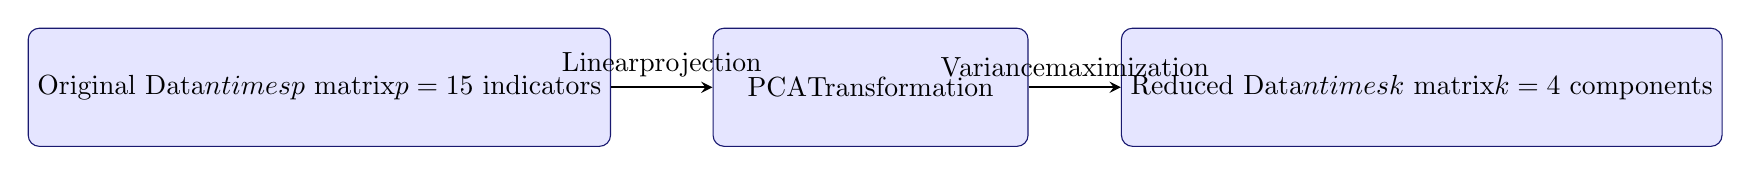
\begin{tikzpicture}[node distance=2cm]
\tikzstyle{block} = [rectangle, rounded corners, minimum width=4cm, minimum height=1.5cm, text centered, draw=MidnightBlue, fill=blue!10]
\tikzstyle{arrow} = [thick,->,>=stealth]

\node (input) [block] {Original Data\\$n \\times p$ matrix\\$p = 15$ indicators};
\node (pca) [block, right of=input, xshift=5cm] {PCA\\Transformation};
\node (output) [block, right of=pca, xshift=5cm] {Reduced Data\\$n \\times k$ matrix\\$k = 4$ components};

\draw [arrow] (input) -- (pca) node[midway, above] {Linear\\projection};
\draw [arrow] (pca) -- (output) node[midway, above] {Variance\\maximization};
\end{tikzpicture}
\end{center}

\begin{block}{Key Mathematical Objective}
Find an orthonormal basis (principal components) that maximizes the variance of the projected data, ordered by decreasing variance.
\end{block}
\end{frame}

\begin{frame}{Geometric Interpretation of PCA}
PCA can be understood as finding the directions of maximum variance in the data:

\begin{center}
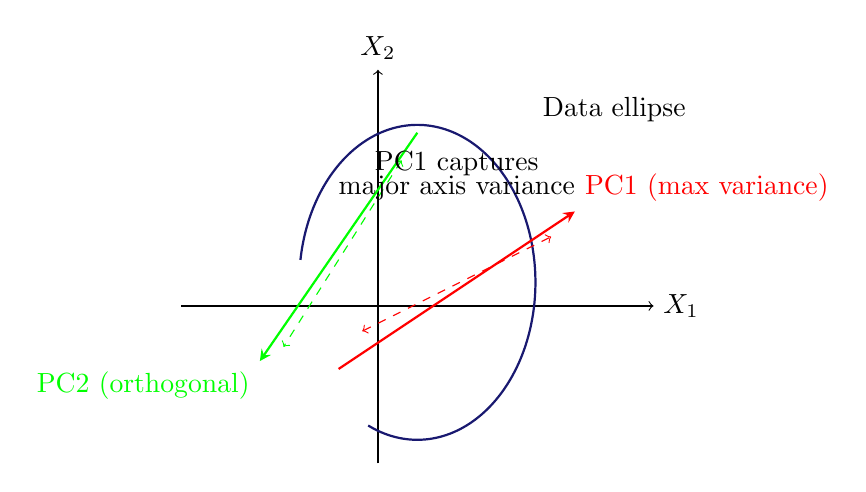
\begin{tikzpicture}[domain=-2:3, smooth, samples=100]
\draw[->] (-2.5,0) -- (3.5,0) node[right] {$X_1$};
\draw[->] (0,-2) -- (0,3) node[above] {$X_2$};

% Ellipse representing correlated data
\draw[thick, MidnightBlue] plot ({1.5*cos(deg(\x)) + 0.5}, {2*sin(deg(\x)) + 0.3});

% Principal components
\draw[->, thick, red, >=stealth] (-0.5,-0.8) -- (2.5,1.2) node[above right] {PC1 (max variance)};
\draw[->, thick, green, >=stealth] (0.5,2.2) -- (-1.5,-0.7) node[below left] {PC2 (orthogonal)};

% Variance arrows
\draw[<->, dashed, red] (-0.2,-0.32) -- (2.2,0.88);
\draw[<->, dashed, green] (0.3,1.85) -- (-1.2,-0.52);

\node at (3,2.5) {Data ellipse};
\node at (1,1.8) {PC1 captures};
\node at (1,1.5) {major axis variance};
\end{tikzpicture}
\end{center}

\begin{block}{Geometric Principles}
\begin{columns}
\begin{column}{0.5\textwidth}
\begin{block}{PC1 (First Component)}
The direction that captures the maximum variance in the data (major axis of the ellipse).
\end{block}
\end{column}
\begin{column}{0.5\textwidth}
\begin{block}{PC2 (Second Component)}
Orthogonal to PC1, captures remaining maximum variance (minor axis).
\end{block}
\end{column}
\end{columns}
\end{block}
\end{frame}

\begin{frame}{Mathematical Formulation of PCA}
The goal of PCA is to find a linear transformation that maximizes variance:

\begin{block}{Data Matrix}
Let $\mathbf{X}$ be an $n \times p$ data matrix where:
\begin{itemize}
\item $n$: Number of observations (patients)
\item $p$: Number of variables (15 clinical indicators)
\end{itemize}
\end{block}

\begin{block}{Principal Components as Linear Combinations}
Each principal component $PC_j$ is a linear combination of the original variables:
$$PC_j = a_{j1}X_1 + a_{j2}X_2 + \cdots + a_{jp}X_p$$
where $\mathbf{a}_j = (a_{j1}, \ldots, a_{jp})$ is the loading vector (eigenvector).
\end{block}

\begin{block}{Optimization Criterion}
Find orthonormal vectors $\mathbf{a}_1, \ldots, \mathbf{a}_k$ such that:
$$\mathbf{a}_j^T \mathbf{a}_j = 1 \quad \text{and} \quad \mathbf{a}_j^T \mathbf{a}_m = 0 \text{ for } j \neq m$$
while maximizing $\text{Var}(\mathbf{X}\mathbf{a}_j)$.
\end{block}
\end{frame}

% ============================================================================
% SECTION 2: MOTIVATION FOR DIMENSIONALITY REDUCTION
% ============================================================================

\section{Motivation for Dimensionality Reduction in Clinical Data}

\subsection{Challenges with High-Dimensional Clinical Data}

\begin{frame}{The Problem of Dimensionality in Clinical Research}
Modern clinical studies often collect numerous measurements per patient:

\begin{center}
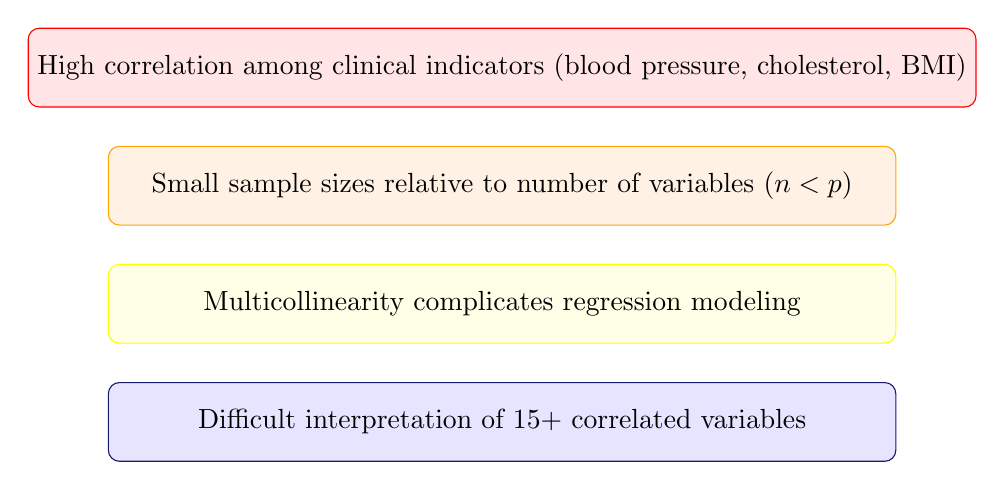
\begin{tikzpicture}[node distance=1.5cm]
\tikzstyle{challenge} = [rectangle, rounded corners, minimum width=10cm, minimum height=1cm, text centered]

\node (C1) [challenge, draw=Red, fill=red!10] {High correlation among clinical indicators (blood pressure, cholesterol, BMI)};
\node (C2) [challenge, below of=C1, draw=Orange, fill=orange!10] {Small sample sizes relative to number of variables ($n < p$)};
\node (C3) [challenge, below of=C2, draw=Yellow, fill=yellow!10] {Multicollinearity complicates regression modeling};
\node (C4) [challenge, below of=C3, draw=MidnightBlue, fill=blue!10] {Difficult interpretation of 15+ correlated variables};
\end{tikzpicture}
\end{center}
\end{frame}

\begin{frame}{Clinical Example: Cardiovascular Risk Assessment}
Consider a cardiovascular risk study with 15 clinical indicators:

\begin{center}
\begin{tabular}{lp{6cm}}
\toprule
Category & Clinical Indicators \\
\midrule
Blood Pressure & Systolic BP, Diastolic BP, Pulse Pressure \\
Lipid Profile & Total Cholesterol, LDL, HDL, Triglycerides \\
Metabolic & Fasting Glucose, HbA1c, BMI, Waist Circumference \\
Inflammatory & CRP, ESR, WBC Count \\
Cardiac Function & Heart Rate, Ejection Fraction \\
Renal Function & Creatinine, eGFR \\
\bottomrule
\end{tabular}
\end{center}

\begin{block}{Challenges}
\begin{itemize}
\item Many indicators are highly correlated (e.g., systolic BP and pulse pressure)
\item Potential for overfitting in predictive models
\item Difficulty communicating findings to clinicians
\end{itemize}
\end{block}
\end{frame}

\begin{frame}{Benefits of Dimensionality Reduction}
Reducing 15 indicators to 4 principal components offers several advantages:

\begin{center}
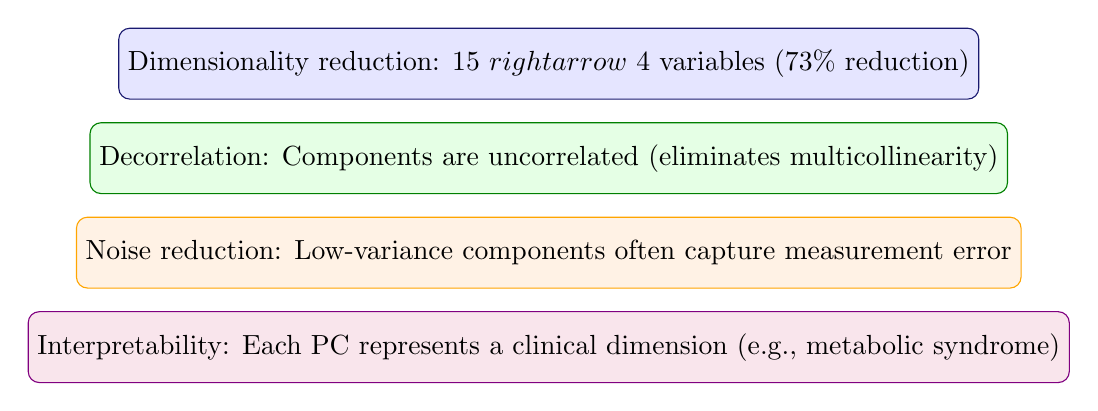
\begin{tikzpicture}[node distance=1.2cm]
\tikzstyle{benefit} = [rectangle, rounded corners, minimum width=10cm, minimum height=0.9cm, text centered]

\node (B1) [benefit, draw=MidnightBlue, fill=blue!10] {Dimensionality reduction: 15 $\\rightarrow$ 4 variables (73\% reduction)};
\node (B2) [benefit, below of=B1, draw=Green, fill=green!10] {Decorrelation: Components are uncorrelated (eliminates multicollinearity)};
\node (B3) [benefit, below of=B2, draw=Orange, fill=orange!10] {Noise reduction: Low-variance components often capture measurement error};
\node (B4) [benefit, below of=B3, draw=Purple, fill=purple!10] {Interpretability: Each PC represents a clinical dimension (e.g., metabolic syndrome)};
\end{tikzpicture}
\end{center}
\end{frame}

\begin{frame}{Applications of PCA in Clinical Research}
PCA has numerous applications in medical research:

\begin{columns}
\begin{column}{0.5\textwidth}
\begin{block}{Data Preprocessing}
\begin{itemize}
\item Feature reduction before classification
\item Creating composite scores
\end{itemize}
\end{block}
\end{column}
\begin{column}{0.5\textwidth}
\begin{block}{Pattern Discovery}
\begin{itemize}
\item Identifying patient subgroups
\end{itemize}
\end{block}
\end{column}
\end{columns}

\begin{block}{Example Applications}
\begin{center}
\begin{tabular}{ll}
\toprule
Application & Description \\
\midrule
Metabolic syndrome & Combining correlated metabolic markers \\
Gene expression & Reducing thousands of genes to interpretable patterns \\
Medical imaging & Dimensionality reduction of MRI/CT features \\
Survey data & Creating composite health status scores \\
\bottomrule
\end{tabular}
\end{center}
\end{block}
\end{frame}

% ============================================================================
% SECTION 3: STEP-BY-STEP IMPLEMENTATION
% ============================================================================

\section{Step-by-Step PCA Implementation}

\subsection{Step 1: Data Standardization}

\begin{frame}{Data Standardization: Why It Matters}
Before performing PCA, variables must be standardized:

\begin{block}{The Problem of Scale Differences}
Clinical indicators often have different scales:
\begin{center}
\begin{tabular}{lrr}
\toprule
Variable & Range & Units \\
\midrule
Systolic BP & 90 - 200 & mmHg \\
Total Cholesterol & 150 - 300 & mg/dL \\
Creatinine & 0.5 - 3.0 & mg/dL \\
HbA1c & 4.0 - 14.0 & \% \\
\bottomrule
\end{tabular}
\end{center}
Without standardization, variables with larger scales would dominate the analysis.
\end{block}

\begin{block}{Standardization Formula}
For each variable $X_j$:
$$Z_{ij} = \frac{X_{ij} - \bar{X}_j}{s_j}$$
where $\bar{X}_j$ is the mean and $s_j$ is the standard deviation.
\end{block}

\begin{block}{Result}
After standardization, each variable has mean 0 and variance 1:
$$\bar{Z}_j = 0, \quad s_Z^2 = 1$$
\end{block}
\end{frame}

\begin{frame}{Standardization in Practice}
The standardized data matrix $\mathbf{Z}$ is used for PCA:

\begin{block}{Standardized Data Matrix}
$$\mathbf{Z} = \begin{bmatrix}
z_{11} & z_{12} & \cdots & z_{1p} \\
z_{21} & z_{22} & \cdots & z_{2p} \\
\vdots & \vdots & \ddots & \vdots \\
z_{n1} & z_{n2} & \cdots & z_{np}
\end{bmatrix}$$
where $p = 15$ clinical indicators and $n$ is the number of patients.
\end{block}

\begin{block}{Properties of Standardized Data}
\begin{itemize}
\item Each column has mean 0
\item Each column has variance 1
\item The covariance matrix equals the correlation matrix
\end{itemize}
\end{block}
\end{frame}

\subsection{Step 2: Covariance and Correlation Matrices}

\begin{frame}{Computing the Covariance Matrix}
The covariance matrix captures the relationships between variables:

\begin{block}{Sample Covariance Matrix Definition}
For standardized data $\mathbf{Z}$:
$$\mathbf{S} = \frac{1}{n-1} \mathbf{Z}^T \mathbf{Z}$$
where $\mathbf{S}$ is a $p \times p$ symmetric matrix.
\end{block}

\begin{block}{Covariance Matrix Elements}
$$s_{jk} = \frac{1}{n-1} \sum_{i=1}^{n} (z_{ij} - \bar{z}_j)(z_{ik} - \bar{z}_k)$$
For standardized data, $s_{jk}$ equals the correlation coefficient $r_{jk}$.
\end{block}

\begin{block}{Correlation Matrix (for Standardized Data)}
$$\mathbf{R} = \frac{1}{n-1} \mathbf{Z}^T \mathbf{Z}$$
Since $Z$ is standardized, $\mathbf{S} = \mathbf{R}$.
\end{block}
\end{frame}

\begin{frame}{Example: Correlation Matrix for 15 Clinical Indicators}
The correlation matrix reveals relationships among variables:

\begin{block}{Symmetric Structure}
$$\mathbf{R} = \begin{bmatrix}
1.00 & r_{12} & \cdots & r_{1,15} \\
r_{21} & 1.00 & \cdots & r_{2,15} \\
\vdots & \vdots & \ddots & \vdots \\
r_{15,1} & r_{15,2} & \cdots & 1.00
\end{bmatrix}$$
where $r_{jk} = r_{kj}$ and diagonal elements are 1.
\end{block}

\begin{block}{Example Correlations in Clinical Data}
\begin{center}
\begin{tabular}{llc}
\toprule
Variable Pair & Interpretation & Correlation \\
\midrule
Systolic BP - Diastolic BP & Strong positive & 0.78 \\
HDL - Triglycerides & Moderate negative & -0.52 \\
Creatinine - eGFR & Strong negative & -0.85 \\
CRP - WBC & Weak positive & 0.23 \\
\bottomrule
\end{tabular}
\end{center}
\end{block}
\end{frame}

\subsection{Step 3: Eigenvalues and Eigenvectors}

\begin{frame}{Eigenvalue Decomposition}
The core of PCA is the eigenvalue decomposition of the covariance matrix:

\begin{block}{Eigenvalue Equation}
Find eigenvalues $\lambda_j$ and eigenvectors $\mathbf{v}_j$ such that:
$$\mathbf{R} \mathbf{v}_j = \lambda_j \mathbf{v}_j$$
where $\mathbf{v}_j^T \mathbf{v}_j = 1$ and $\mathbf{v}_j^T \mathbf{v}_k = 0$ for $j \neq k$.
\end{block}

\begin{block}{Eigen Decomposition}
The full decomposition is:
$$\mathbf{R} = \mathbf{V} \boldsymbol{\Lambda} \mathbf{V}^T$$
where:
\begin{itemize}
\item $\mathbf{V} = [\mathbf{v}_1, \mathbf{v}_2, \ldots, \mathbf{v}_{15}]$: Orthogonal matrix of eigenvectors
\item $\boldsymbol{\Lambda} = \text{diag}(\lambda_1, \lambda_2, \ldots, \lambda_{15})$: Diagonal matrix of eigenvalues
\end{itemize}
\end{block}

\begin{block}{Properties}
\begin{itemize}
\item Eigenvalues $\lambda_j \geq 0$ (since $\mathbf{R}$ is positive semi-definite)
\item Eigenvectors are orthonormal: $\mathbf{V}^T \mathbf{V} = \mathbf{I}$
\end{itemize}
\end{block}
\end{frame}

\begin{frame}{Eigenvalues as Variance Explained}
Each eigenvalue represents the variance explained by its corresponding principal component:

\begin{block}{Variance Interpretation}
For standardized data:
$$\lambda_j = \text{Var}(PC_j) = \text{Var}(\mathbf{Z}\mathbf{v}_j)$$
The sum of all eigenvalues equals the total variance:
$$\sum_{j=1}^{15} \lambda_j = p = 15$$
\end{block}

\begin{block}{Example Eigenvalue Spectrum}
\begin{center}
\begin{tabular}{cccc}
\toprule
Component & Eigenvalue ($\lambda_j$) & Variance \% & Cumulative \% \\
\midrule
PC1 & 4.52 & 30.1 & 30.1 \\
PC2 & 2.87 & 19.1 & 49.2 \\
PC3 & 2.14 & 14.3 & 63.5 \\
PC4 & 1.68 & 11.2 & 74.7 \\
PC5 & 1.23 & 8.2 & 82.9 \\
$\vdots$ & $\vdots$ & $\vdots$ & $\vdots$ \\
PC15 & 0.21 & 1.4 & 100.0 \\
\bottomrule
\end{tabular}
\end{center}
\end{block}
\end{frame}

\begin{frame}{Eigenvectors as Loading Vectors}
Eigenvectors contain the loadings that define each principal component:

\begin{block}{Loading Matrix}
The eigenvector matrix $\mathbf{V}$ contains the loadings:
$$\mathbf{V} = \begin{bmatrix}
v_{11} & v_{12} & v_{13} & v_{14} \\
v_{21} & v_{22} & v_{23} & v_{24} \\
\vdots & \vdots & \vdots & \vdots \\
v_{15,1} & v_{15,2} & v_{15,3} & v_{15,4}
\end{bmatrix}$$
Each column represents the loadings for one principal component.
\end{block}

\begin{block}{Loadings Interpretation}
The loading $v_{kj}$ represents the contribution of variable $X_k$ to principal component $PC_j$:
$$PC_j = v_{1j}X_1 + v_{2j}X_2 + \cdots + v_{15,j}X_{15}$$
\end{block}

\begin{block}{Squared Loadings}
The squared loading $v_{kj}^2$ represents the proportion of variance in $PC_j$ attributable to variable $X_k$:
$$\sum_{k=1}^{15} v_{kj}^2 = \lambda_j$$
\end{block}
\end{frame}

\begin{frame}{Step-by-Step Algorithm Summary}
\begin{center}
\begin{tikzpicture}[node distance=1cm]
\tikzstyle{step} = [rectangle, rounded corners, minimum width=12cm, minimum height=0.9cm, text centered]

\node (S1) [step, draw=MidnightBlue, fill=blue!10] {\textbf{Step 1:} Standardize data: $Z_{ij} = (X_{ij} - \\bar{X}_j) / s_j$};
\node (S2) [step, below of=S1, draw=Green, fill=green!10] {\textbf{Step 2:} Compute covariance (correlation) matrix: $\\mathbf{R} = \\frac{1}{n-1}\\mathbf{Z}^T\\mathbf{Z}$};
\node (S3) [step, below of=S2, draw=Orange, fill=orange!10] {\textbf{Step 3:} Eigenvalue decomposition: $\\mathbf{R}\\mathbf{v}_j = \\lambda_j\\mathbf{v}_j$};
\node (S4) [step, below of=S3, draw=Purple, fill=purple!10] {\textbf{Step 4:} Order by eigenvalues: $\\lambda_1 \\geq \\lambda_2 \\geq \\cdots \\geq \\lambda_{15}$};
\node (S5) [step, below of=S4, draw=Red, fill=red!10] {\textbf{Step 5:} Select top $k$ components and compute scores: $\\mathbf{PC} = \\mathbf{Z}\\mathbf{V}_k$};
\end{tikzpicture}
\end{center}
\end{frame}

% ============================================================================
% SECTION 4: VARIANCE EXPLAINED AND COMPONENT SELECTION
% ============================================================================

\section{Variance Explained and Component Selection}

\subsection{Calculating and Interpreting Variance Explained}

\begin{frame}{Variance Explained: The Key Metric}
The proportion of variance explained guides component selection:

\begin{block}{Variance Explained by Component $j$}
$$\text{VE}_j = \frac{\lambda_j}{\sum_{m=1}^{p} \lambda_m} \times 100\%$$
For standardized data, $\sum \lambda_m = p = 15$.
\end{block}

\begin{block}{Cumulative Variance Explained}
$$\text{CVE}_k = \sum_{j=1}^{k} \text{VE}_j \times 100\%$$
This represents the total variance captured by the first $k$ components.
\end{block}

\begin{block}{Example Calculation}
For our clinical data:
\begin{align*}
\text{VE}_1 &= \frac{4.52}{15} \times 100\% = 30.1\% \\
\text{VE}_2 &= \frac{2.87}{15} \times 100\% = 19.1\% \\
\text{VE}_3 &= \frac{2.14}{15} \times 100\% = 14.3\% \\
\text{VE}_4 &= \frac{1.68}{15} \times 100\% = 11.2\% \\
\text{CVE}_4 &= 30.1 + 19.1 + 14.3 + 11.2 = 74.7\%
\end{align*}
\end{block}
\end{frame}

\begin{frame}{Scree Plot for Component Selection}
The scree plot visualizes eigenvalues to guide component selection:

\begin{center}
\begin{tikzpicture}[domain=0.5:15.5, samples=15]
\draw[->] (0,0) -- (16,0) node[right] {Component Number};
\draw[->] (0,0) -- (0,5) node[above] {Eigenvalue};

% Eigenvalue data points
\draw[thick, MidnightBlue, mark=*, mark size=3pt] plot coordinates {
(1,4.52)
(2,2.87)
(3,2.14)
(4,1.68)
(5,1.23)
(6,0.95)
(7,0.72)
(8,0.58)
(9,0.45)
(10,0.35)
(11,0.28)
(12,0.24)
(13,0.21)
(14,0.18)
(15,0.15)
};

% Kaiser criterion line
\draw[dashed, red] (0,1) -- (16,1) node[right at={(16,1)}] {Kaiser criterion ($\\lambda=1$)};

% Elbow
\node[circle, draw=Red, fill=red!10, minimum size=0.3cm] at (4,1.68) {};

\node at (10,4) {Scree Plot};
\node at (10,3.5) {Elbow at PC4};
\end{tikzpicture}
\end{center}

\begin{block}{Selection Criteria}
\begin{center}
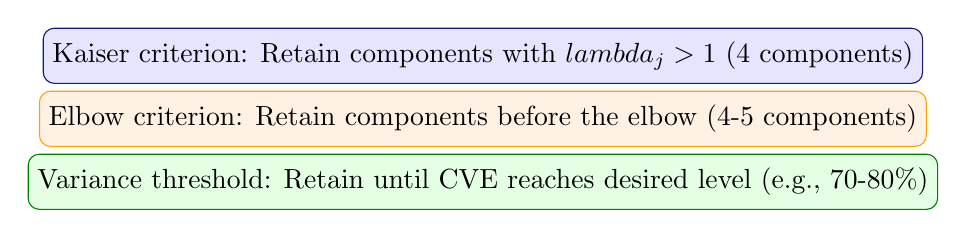
\begin{tikzpicture}[node distance=0.8cm]
\tikzstyle{criteria} = [rectangle, rounded corners, minimum width=10cm, minimum height=0.7cm, text centered]

\node (C1) [criteria, draw=MidnightBlue, fill=blue!10] {Kaiser criterion: Retain components with $\\lambda_j > 1$ (4 components)};
\node (C2) [criteria, below of=C1, draw=Orange, fill=orange!10] {Elbow criterion: Retain components before the elbow (4-5 components)};
\node (C3) [criteria, below of=C2, draw=Green, fill=green!10] {Variance threshold: Retain until CVE reaches desired level (e.g., 70-80\%)};
\end{tikzpicture}
\end{center}
\end{block}
\end{frame}

\begin{frame}{Justifying 4 Principal Components}
Several criteria support selecting 4 components from 15:

\begin{block}{Kaiser Criterion}
Retain components with eigenvalue > 1:
\begin{itemize}
\item PC1: $\lambda_1 = 4.52 > 1$ ✓
\item PC2: $\lambda_2 = 2.87 > 1$ ✓
\item PC3: $\lambda_3 = 2.14 > 1$ ✓
\item PC4: $\lambda_4 = 1.68 > 1$ ✓
\item PC5: $\lambda_5 = 1.23 > 1$ (borderline)
\end{itemize}
\end{block}

\begin{block}{Cumulative Variance}
4 components explain 74.7\% of total variance, which exceeds the commonly recommended 70-75\% threshold.
\end{block}

\begin{block}{Practical Considerations}
73\% reduction (15 → 4 variables) while retaining substantial information is often acceptable in clinical research.
\end{block}
\end{frame}

% ============================================================================
% SECTION 5: INTERPRETATION OF PRINCIPAL COMPONENTS
% ============================================================================

\section{Interpreting Principal Components in Clinical Context}

\subsection{Understanding Component Structure}

\begin{frame}{Interpreting Principal Components}
Each principal component represents a clinical dimension:

\begin{block}{Loading Interpretation}
High loadings (absolute value > 0.3-0.4) indicate variables strongly associated with a component:
\begin{center}
\begin{tabular}{lc}
\toprule
Variable & Loading on PC1 \\
\midrule
Systolic BP & 0.42 \\
Diastolic BP & 0.38 \\
Pulse Pressure & 0.41 \\
LDL Cholesterol & 0.28 \\
HDL Cholesterol & -0.15 \\
\hline
Interpretation & PC1 represents blood pressure burden \\
\bottomrule
\end{tabular}
\end{center}
\end{block}

\begin{block}{Communality}
The proportion of variance in each variable explained by the retained components:
$$h_k^2 = \sum_{j=1}^{4} v_{kj}^2$$
Variables with low communality (< 0.5) are not well-represented by the components.
\end{block}
\end{frame}

\begin{frame}{Example Component Interpretation}
For our 15 clinical indicators, the 4 components might represent:

\begin{center}
\begin{tabular}{lp{8cm}c}
\toprule
Component & Clinical Interpretation & Variance \% \\
\midrule
PC1 & \textbf{Cardiovascular Risk}: Systolic BP, Diastolic BP, Pulse Pressure, LDL, Triglycerides & 30.1 \\
\midrule
PC2 & \textbf{Metabolic Syndrome}: BMI, Waist Circumference, Fasting Glucose, HbA1c & 19.1 \\
\midrule
PC3 & \textbf{Inflammatory Status}: CRP, ESR, WBC Count & 14.3 \\
\midrule
PC4 & \textbf{Renal Function}: Creatinine, eGFR & 11.2 \\
\bottomrule
\end{tabular}
\end{center}

\begin{block}{Total Variance Explained}
Cumulative variance: 74.7\% of the original 15-indicator information is retained in these 4 clinical dimensions.
\end{block}
\end{frame}

\begin{frame}{Computing Principal Component Scores}
Principal component scores are used for subsequent analysis:

\begin{block}{Score Calculation}
For each observation $i$ and component $j$:
$$PC_{ij} = z_{i1}v_{1j} + z_{i2}v_{2j} + \cdots + z_{i,15}v_{15,j}$$
In matrix form: $\mathbf{PC} = \mathbf{Z}\mathbf{V}_4$
\end{block}

\begin{block}{Score Matrix}
$$\mathbf{PC} = \begin{bmatrix}
PC_{11} & PC_{12} & PC_{13} & PC_{14} \\
PC_{21} & PC_{22} & PC_{23} & PC_{24} \\
\vdots & \vdots & \vdots & \vdots \\
PC_{n1} & PC_{n2} & PC_{n3} & PC_{n4}
\end{bmatrix}$$
\end{block}

\begin{block}{Properties of Scores}
\begin{itemize}
\item Each column has mean 0
\item Each column has variance equal to the corresponding eigenvalue
\end{itemize}
\end{block}
\end{frame}

\begin{frame}{Biplot for Joint Interpretation}
The biplot visualizes observations and variables simultaneously:

\begin{center}
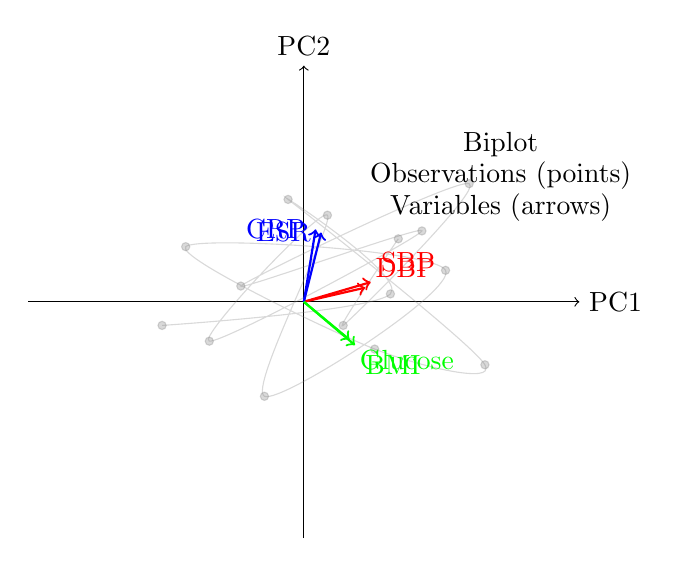
\begin{tikzpicture}[domain=-3:3, smooth, samples=50]
\draw[->] (-3.5,0) -- (3.5,0) node[right] {PC1};
\draw[->] (0,-3) -- (0,3) node[above] {PC2};

% Observations
\draw[gray, opacity=0.3, mark=*, mark size=1.5pt] plot coordinates {
(1.2,0.8)
(0.5,-0.3)
(2.1,1.5)
(-0.8,0.2)
(1.5,0.9)
(-1.2,-0.5)
(0.3,1.1)
(-0.5,-1.2)
(1.8,0.4)
(-1.5,0.7)
(0.9,-0.6)
(2.3,-0.8)
(-0.2,1.3)
(1.1,0.1)
(-1.8,-0.3)
};

% Variable loading vectors
\draw[->, thick, red] (0,0) -- (0.85,0.25) node[above right] {SBP};
\draw[->, thick, red] (0,0) -- (0.78,0.18) node[above right] {DBP};
\draw[->, thick, blue] (0,0) -- (0.15,0.92) node[left] {CRP};
\draw[->, thick, blue] (0,0) -- (0.22,0.88) node[left] {ESR};
\draw[->, thick, green] (0,0) -- (0.65,-0.55) node[below right] {BMI};
\draw[->, thick, green] (0,0) -- (0.58,-0.48) node[below right] {Glucose};

\node at (2.5,2) {Biplot};
\node at (2.5,1.6) {Observations (points)};
\node at (2.5,1.2) {Variables (arrows)};
\end{tikzpicture}
\end{center}

\begin{block}{Biplot Interpretation}
\begin{itemize}
\item \textbf{Points}: Patient scores in PC1-PC2 space
\item \textbf{Arrows}: Variable loadings (direction and magnitude)
\end{itemize}
\end{block}
\end{frame}

% ============================================================================
% SECTION 6: LIMITATIONS OF PCA
% ============================================================================

\section{Limitations and Considerations}

\begin{frame}{Limitations of Principal Component Analysis}
PCA has important limitations that must be considered:

\begin{center}
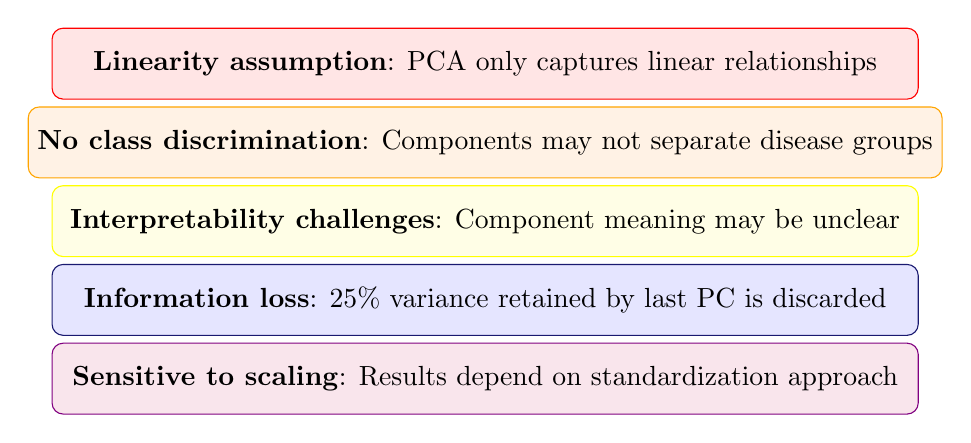
\begin{tikzpicture}[node distance=1cm]
\tikzstyle{limitation} = [rectangle, rounded corners, minimum width=11cm, minimum height=0.9cm, text centered]

\node (L1) [limitation, draw=Red, fill=red!10] {\textbf{Linearity assumption}: PCA only captures linear relationships};
\node (L2) [limitation, below of=L1, draw=Orange, fill=orange!10] {\textbf{No class discrimination}: Components may not separate disease groups};
\node (L3) [limitation, below of=L2, draw=Yellow, fill=yellow!10] {\textbf{Interpretability challenges}: Component meaning may be unclear};
\node (L4) [limitation, below of=L3, draw=MidnightBlue, fill=blue!10] {\textbf{Information loss}: 25\% variance retained by last PC is discarded};
\node (L5) [limitation, below of=L4, draw=Purple, fill=purple!10] {\textbf{Sensitive to scaling}: Results depend on standardization approach};
\end{tikzpicture}
\end{center}
\end{frame}

\begin{frame}{Assumptions and Requirements}
PCA requires certain conditions to be valid:

\begin{block}{Assumptions}
\begin{columns}
\begin{column}{0.5\textwidth}
\begin{block}{Required}
\begin{itemize}
\item Continuous variables
\end{itemize}
\end{block}
\end{column}
\begin{column}{0.5\textwidth}
\begin{block}{Implied}
\begin{itemize}
\item Linear relationships among variables
\end{itemize}
\end{block}
\end{column}
\end{columns}
\end{block}

\begin{block}{Preprocessing Requirements}
\begin{center}
\begin{tabular}{ll}
\toprule
Issue & Solution \\
\midrule
Missing data & Imputation before PCA \\
Outliers & Robust standardization or removal \\
Mixed variable types & Use correlation matrix or Gower distance \\
\bottomrule
\end{tabular}
\end{center}
\end{block}
\end{frame}

\begin{frame}{Alternatives to PCA}
When PCA is inappropriate, consider these alternatives:

\begin{center}
\begin{tabular}{p{4cm}p{6cm}}
\toprule
Method & When to Use \\
\midrule
Kernel PCA & Non-linear relationships \\
Factor Analysis & Latent constructs are hypothesized \\
t-SNE / UMAP & Visualization of high-dimensional data \\
Non-negative Matrix Factorization & Parts-based representation \\
\bottomrule
\end{tabular}
\end{center}

\begin{block}{Choice Considerations}
\begin{itemize}
\item PCA: Maximum variance capture, unsupervised dimensionality reduction
\item Factor Analysis: When latent constructs are hypothesized
\end{itemize}
\end{block}
\end{frame}

% ============================================================================
% SECTION 7: CONCLUSION
% ============================================================================

\section{Conclusion}

\begin{frame}{Summary: PCA Implementation for Clinical Data}
Key steps in implementing PCA for 15 clinical indicators:

\begin{center}
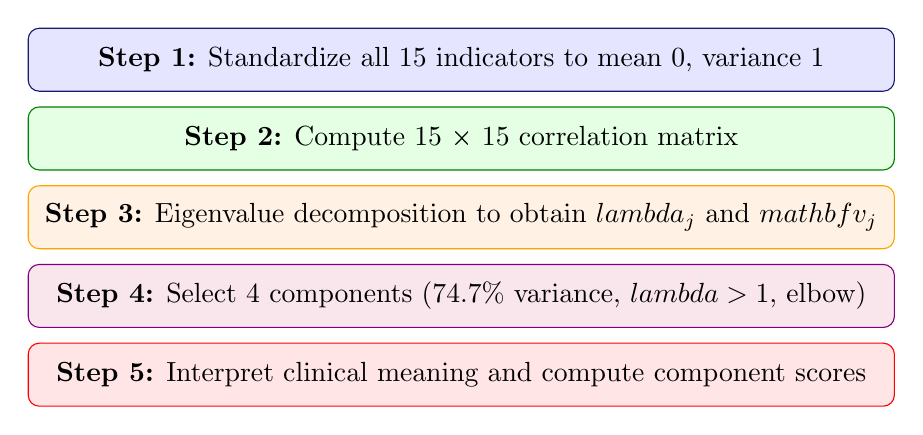
\begin{tikzpicture}[node distance=1cm]
\tikzstyle{summary} = [rectangle, rounded corners, minimum width=11cm, minimum height=0.8cm, text centered]

\node (S1) [summary, draw=MidnightBlue, fill=blue!10] {\textbf{Step 1:} Standardize all 15 indicators to mean 0, variance 1};
\node (S2) [summary, below of=S1, draw=Green, fill=green!10] {\textbf{Step 2:} Compute 15 × 15 correlation matrix};
\node (S3) [summary, below of=S2, draw=Orange, fill=orange!10] {\textbf{Step 3:} Eigenvalue decomposition to obtain $\\lambda_j$ and $\\mathbf{v}_j$};
\node (S4) [summary, below of=S3, draw=Purple, fill=purple!10] {\textbf{Step 4:} Select 4 components (74.7\% variance, $\\lambda > 1$, elbow)};
\node (S5) [summary, below of=S4, draw=Red, fill=red!10] {\textbf{Step 5:} Interpret clinical meaning and compute component scores};
\end{tikzpicture}
\end{center}
\end{frame}

\begin{frame}{Key Equations Summary}
\begin{center}
\begin{small}
\begin{align*}
\textbf{Standardization:} \quad & Z_{ij} = \\frac{X_{ij} - \\bar{X}_j}{s_j} \\\\
\textbf{Correlation Matrix:} \quad & \\mathbf{R} = \\frac{1}{n-1}\\mathbf{Z}^T\\mathbf{Z} \\\\
\textbf{Eigen Decomposition:} \quad & \\mathbf{R}\\mathbf{v}_j = \\lambda_j\\mathbf{v}_j \\\\
\textbf{Variance Explained:} \quad & \\text{VE}_j = \\frac{\\lambda_j}{\\sum_{m=1}^{15}\\lambda_m} \\times 100\\% \\\\
\textbf{Component Scores:} \quad & PC_{ij} = \\sum_{k=1}^{15} z_{ik}v_{kj} \\\\
\textbf{Cumulative Variance:} \quad & \\text{CVE}_4 = \\sum_{j=1}^{4}\\text{VE}_j = 74.7\\%
\end{align*}
\end{small}
\end{center}
\end{frame}

\begin{frame}{Final Takeaways for Clinical Research}
\begin{columns}
\begin{column}{0.5\textwidth}
\begin{block}{Benefits of PCA}
\begin{itemize}
\item Reduces 15 clinical indicators to 4 interpretable dimensions
\end{itemize}
\end{block}
\end{column}
\begin{column}{0.5\textwidth}
\begin{block}{Cautions}
\begin{itemize}
\item Components may not align with clinical constructs
\end{itemize}
\end{block}
\end{column}
\end{columns}

\begin{center}
\textbf{"PCA transforms correlated clinical measurements into orthogonal clinical dimensions, facilitating interpretation and subsequent analysis while preserving the maximum variance in the original data."}
\end{center}
\end{frame}

\begin{frame}{References}
\begin{small}
\begin{itemize}
\item Jolliffe, I.T. and Cadima, J. (2016). Principal component analysis: A review and recent developments. Philosophical Transactions of the Royal Society A, 374(2065), 20150202.
\item Ringnér, M. (2008). What is principal component analysis? Nature Biotechnology, 26(3), 303-304.
\item Hastie, T., Tibshirani, R., and Friedman, J. (2009). The Elements of Statistical Learning: Data Mining, Inference, and Prediction (2nd ed.). Springer.
\end{itemize}
\end{small}
\end{frame}

\end{document}
